% !TeX root = ../proceedings.tex

\section{Design Challenges}
\subsection{Accessibility}
To manoeuvre around in any application, a menu is needed. The menu is something every user has experience with and it is the first thing a user is met with when running an application. This means that the menu has to consist of certain classic elements.\par A user needs a way to close the application. On mobile phones nowadays this can be done with 'return' buttons on the phone, but applications generally have a built in exit function.\par
The user also needs to have some sort of options menu and guidelines. Stacking LEGO seems simple and intuitive, but all the operations and possibilities is something that can confuse a potential user. \par
Lastly it shouldn't be complicated for the user to start a new LEGO session. \par
\subsection{A Main Menu}
To achieve accessibility a '5 plus 5' sketch generation session was held. Initially we thought about this application as a game, therefore the user would typically be met by a main menu screen, just as figure \ref{fig:menu8} illustrates.
\begin{figure}[h]
	\centering
	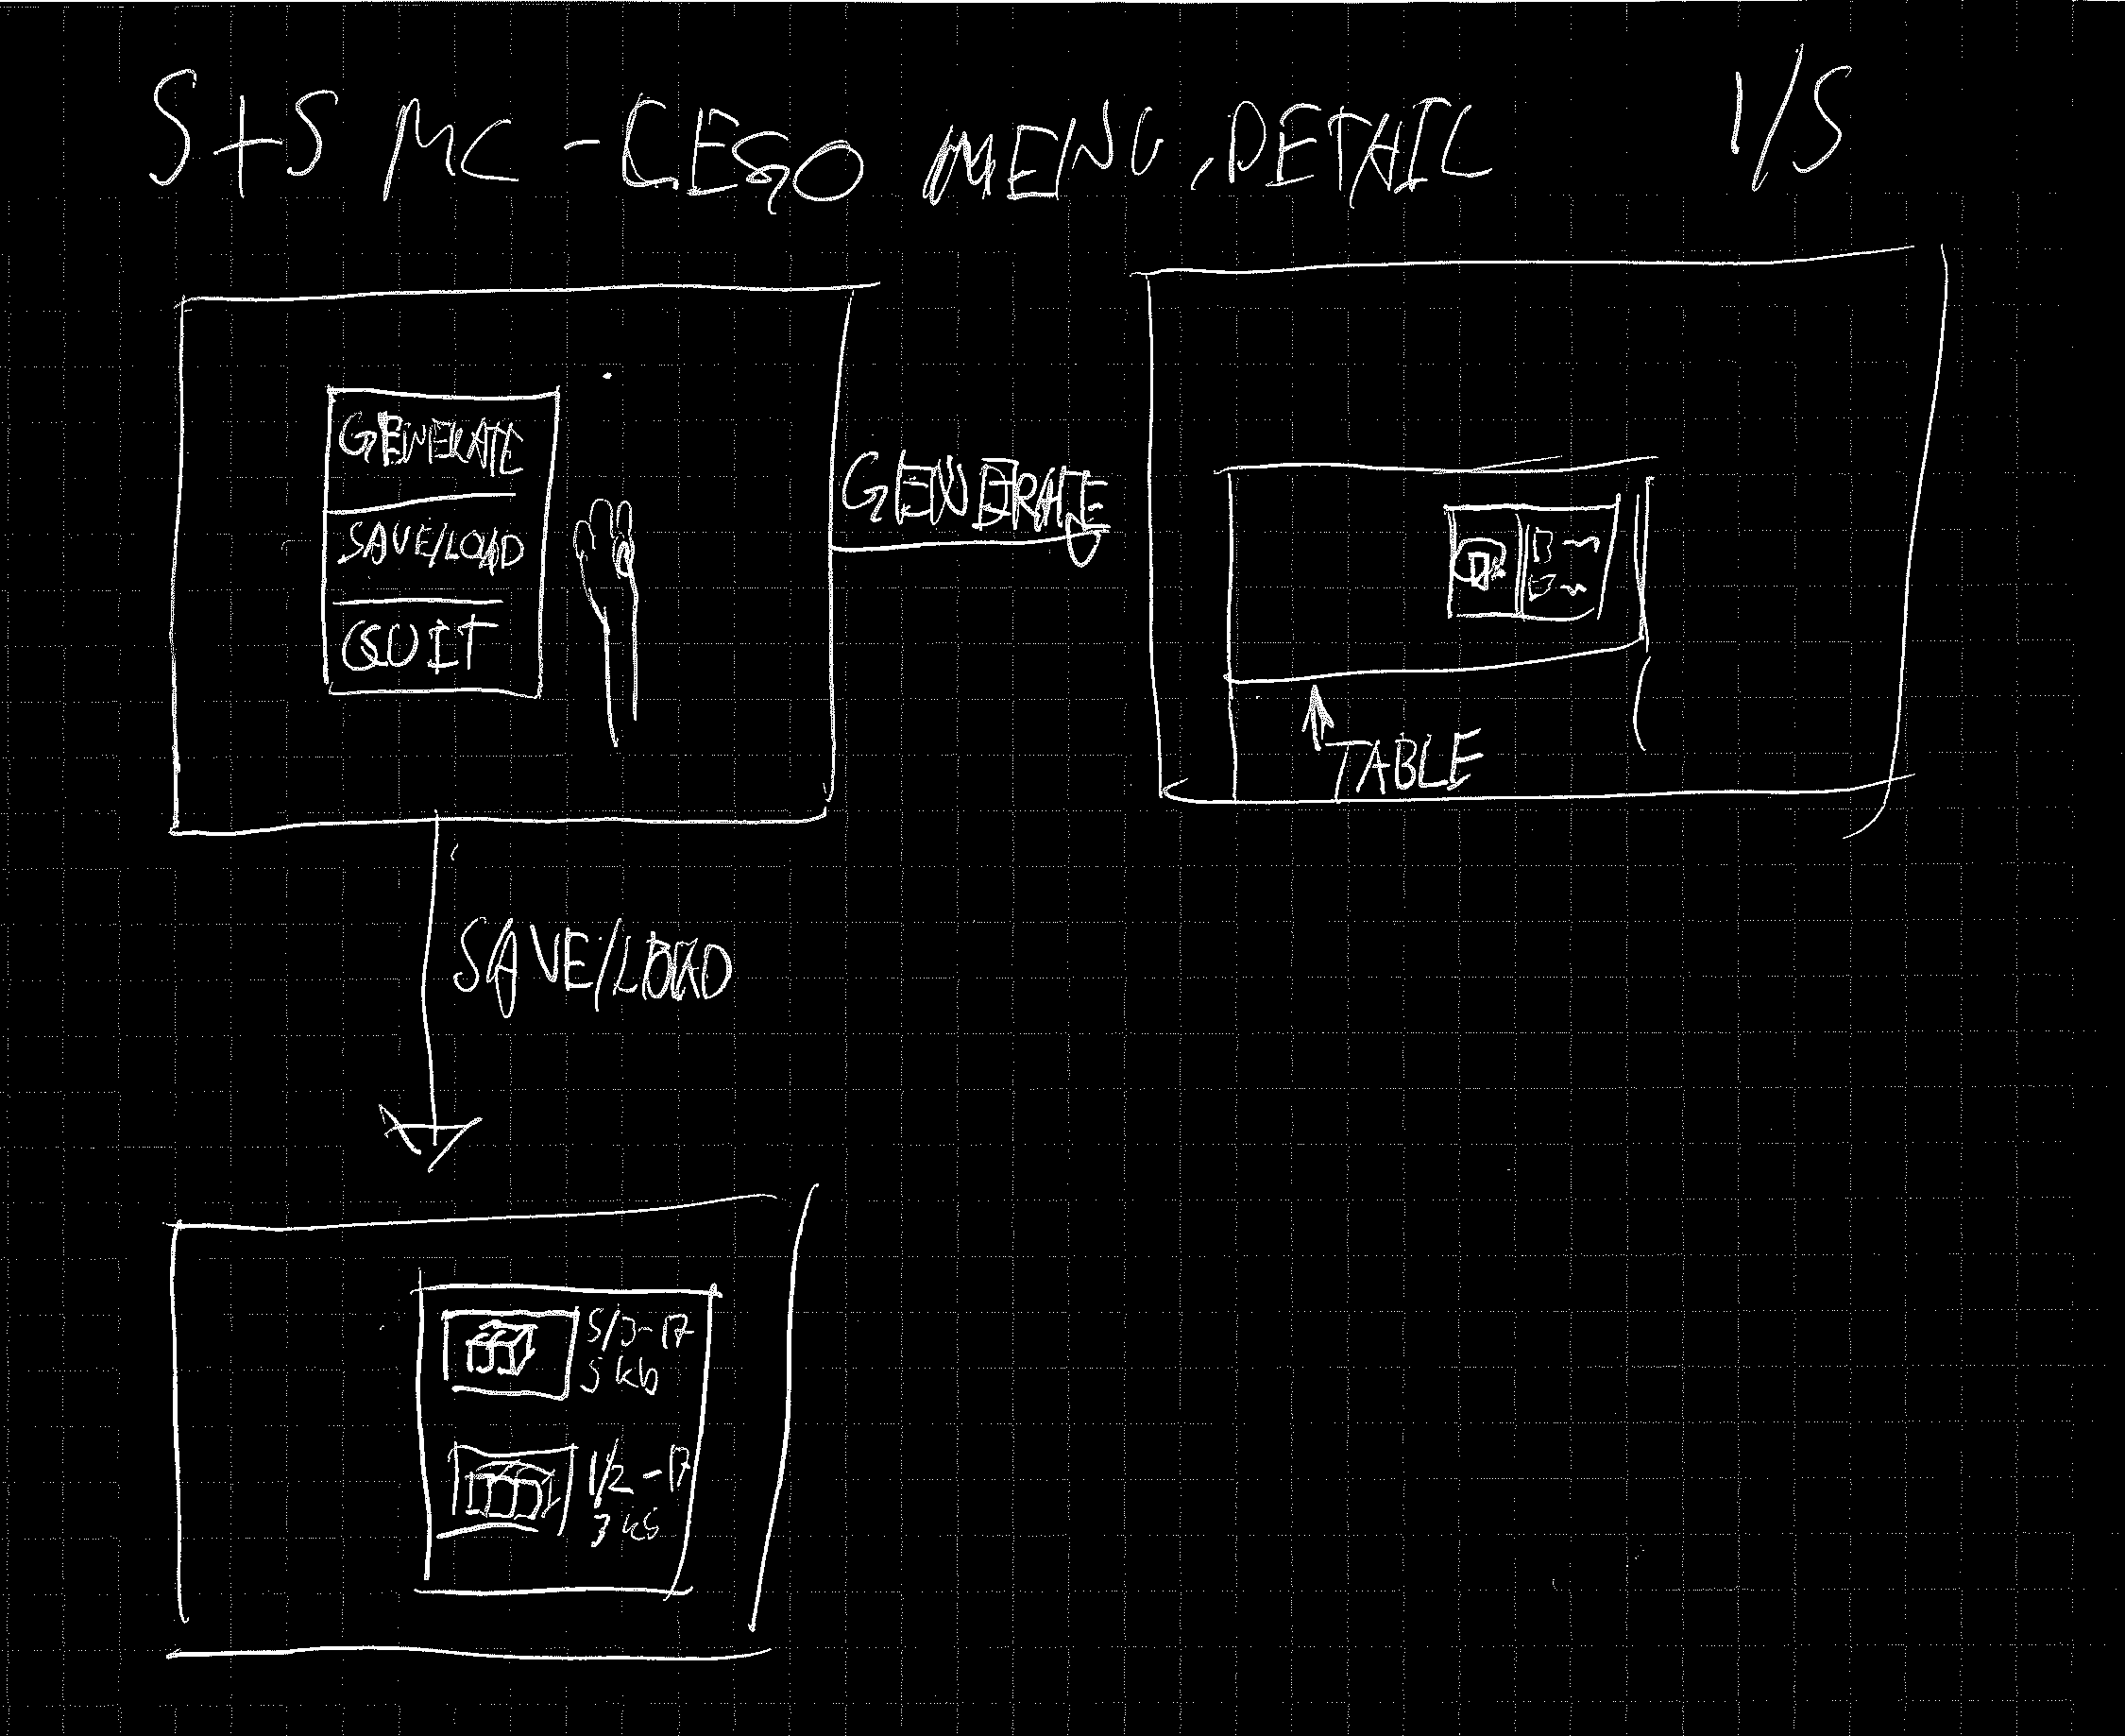
\includegraphics[width=0.7\linewidth]{figures/Menu/menu8}
	\caption{The first idea of a seperate Main Menu screen}
	\label{fig:menu8}
\end{figure}
The user would open the Hololens application, and be met with a menu screen, where actions such as generating a play area, loading and saving a game and a way to quit the application were possible. \par
One common theme in the sketching of the main menu was separating the design of the menu and the interaction techniques with the menu. This led to some sketches being focused on the interaction, such as figure \ref{fig:menugesture} depicts, and other sketches that solely focused on the menu design.\par
\begin{figure}[h]
	\centering
	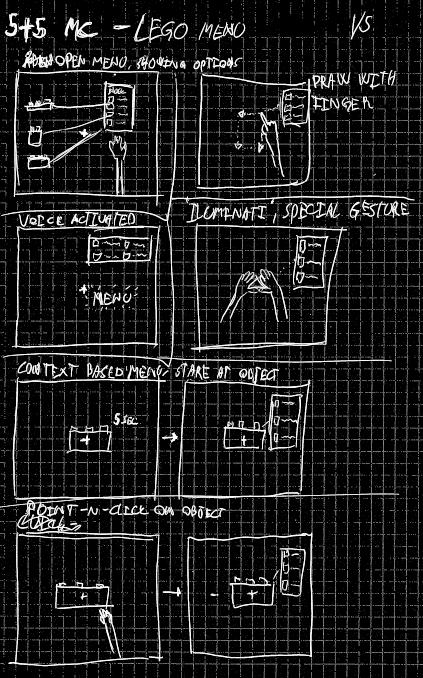
\includegraphics[width=0.7\linewidth]{figures/Menu/menu5}
	\caption{A focus on gestures rather than design, impacted the design. The figure shows 5 different ways of creating an interactive menu for the user to use.}
	\label{fig:menugesture}
\end{figure}
\par
The possibilities with the HoloLens gestures and the augmented reality made it apparent that the menu had to be movable, either by closing and opening with the gestures available, or being able to move it around the play area. 
\subsection{The Generator Board}
After discussing menus in the context of the Hololens, it became apparent that there was a need for a menu that could be placed and interacted within the real world. This menu should only interact inside the play area, and have functions tied to the bricks. Figure \ref{fig:genboard1} is a sketch of what functionalities the generator board could have.
\begin{figure}[h]
	\centering
	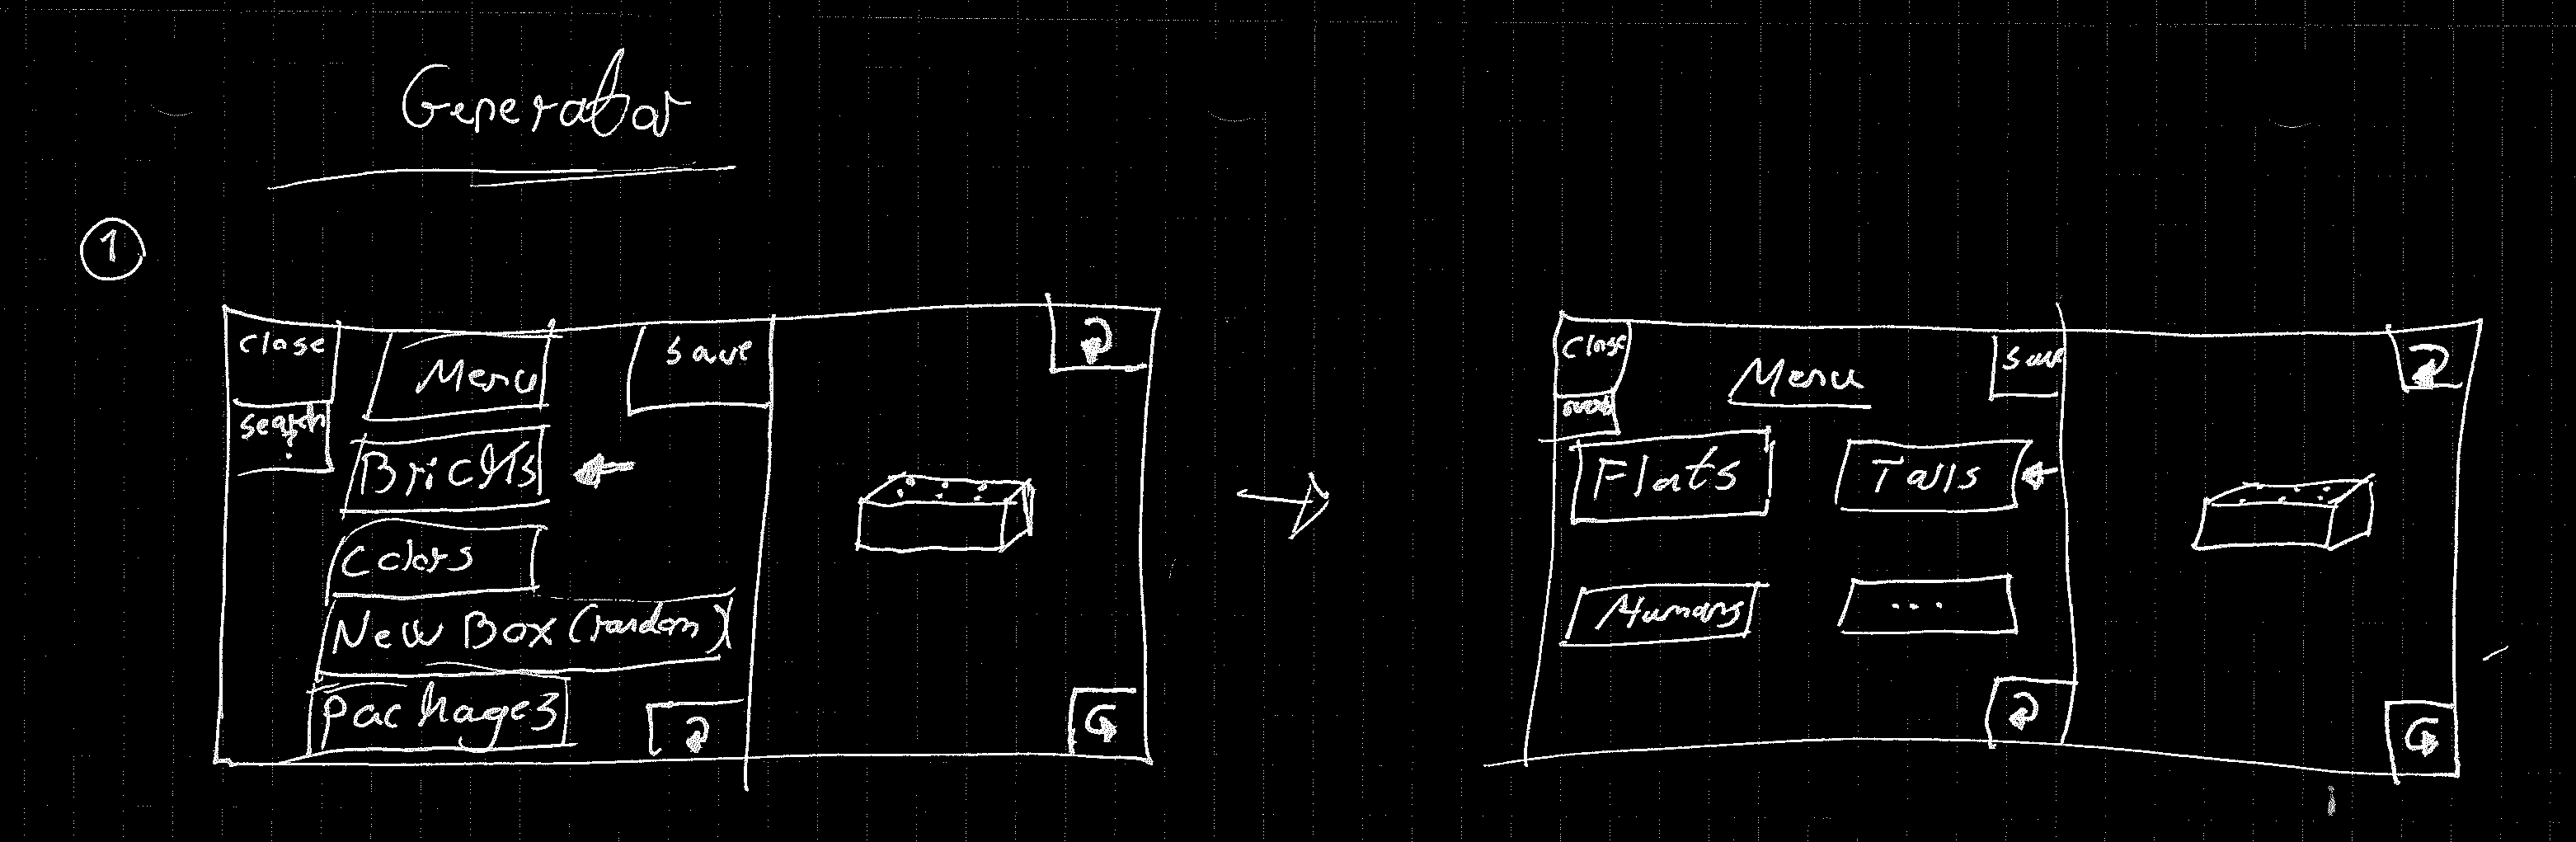
\includegraphics[width=0.7\columnwidth]{figures/Generator/gen5.png}
	\caption{An initial sketch of how the generator board could look like. The menu screen has alot of functionalities, and the actions chosen happen on the right side.}~\label{fig:genboard1}
\end{figure}
The generator board should be have functionalites that can alter the blocks, but also needs to be interactive and moveable in the play area.\par
Figure \ref{fig:gentablet} illustrates how the generator board is placed on a table and used for generating bricks.
\begin{figure}[h]
	\centering
	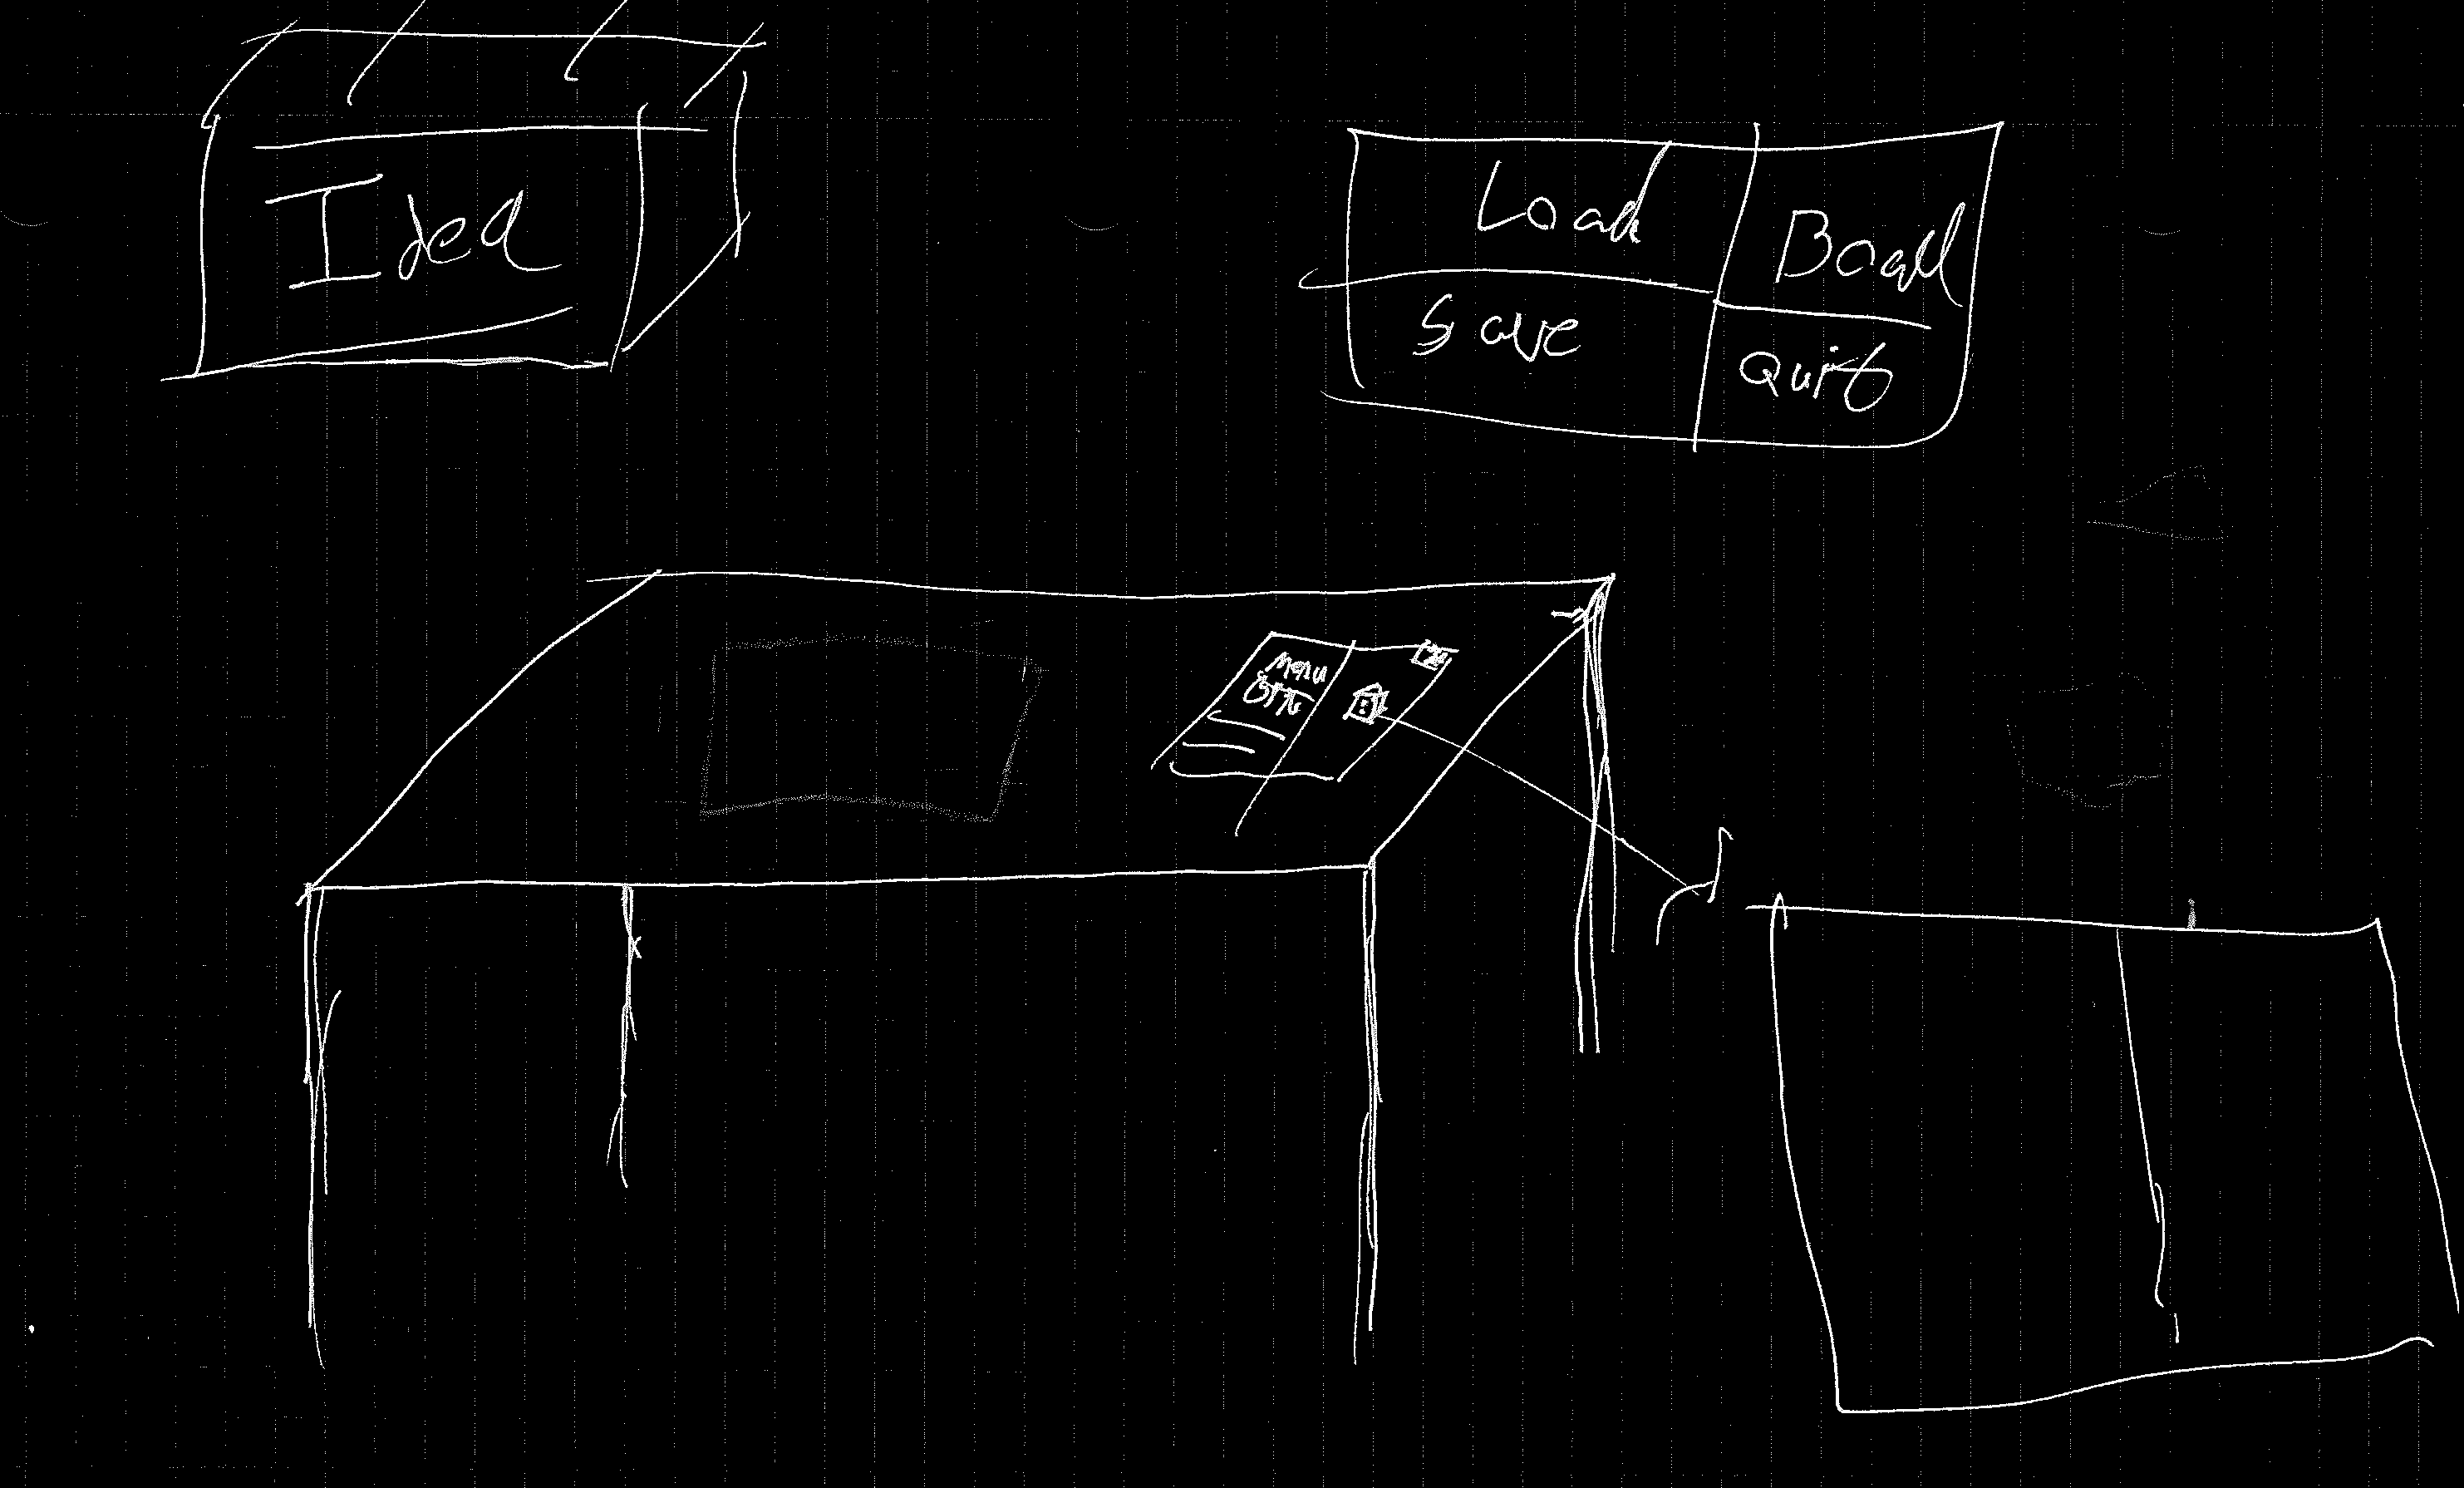
\includegraphics[width=0.7\columnwidth]{figures/Generator/gen6.png}
	\caption{First sketch of the generator board as a movable object. Here placed on the table, spawning blocks on the table.}~\label{fig:gentablet}
\end{figure}
We designed the generator board as a tablet device. Being a solid familar object, makes it more intuitive and natural for the user to interact with. To lift, move and place the tablet on a surface is a simple and familiar task for the user. To accompany the tablet device, a simple interface was designed. The interface only needed simple function all tied to spawning lego bricks. The user can spawn bricks of different types, change colors and saving/loading a play scene.
\subsection{Design Decisions}
\begin{figure}[h]
	\centering
	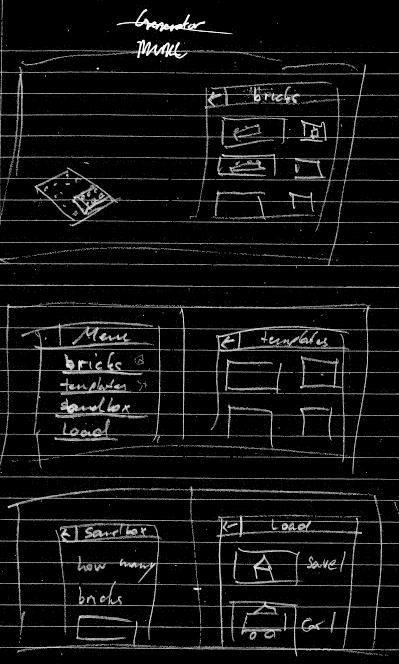
\includegraphics[width=0.5\columnwidth]{figures/Menu/menu1.png}
	\caption{Initial Main Menu screen with big buttons, simple interaction and short descriptions.}~\label{fig:genboard}
\end{figure}
During the sketching phase, several design choices were discussed. One of the very first concerns was the overall look of the main menu. The choice of big buttons, clear visual cues and short textual descriptions was present in almost all of the sketches in the early design phase, as seen in figure \ref{fig:genboard}. The generator board needed to have the same simple design. We decided The menus should not be overcomplicated, but not sparse in functions either.\par
As the development of the application progressed it became more  apparent that an actual main menu was not necessary. All the interactions needed for the prototype could be implemented  the tablet looking generator board and could ease user interaction with the application. Instead of going through a main menu and then having the generator which contains the functionality for working with the LEGO bricks, spawning the generator board at the application start up and "cutting out the middleman" seemed as a natural choice for this prototype. Granted, with an eventual increase in functionality and complexity of the application, a root/main menu might prove useful as to not clutter the users experience when they are building as opposed to when they are in the main menu setting options, loading scenarios, downloading templates etc. 

